\section{Applied 2019: Solution\footnote{Nikos Ignatiadis and D.K.}}



\subsection*{Problem 1: Analyzing a randomized clinical trial}

Key ideas/tools:
\begin{itemize}
  \item log-rank (Mantel-Haenszel) test
  \item Cox proportional hazards model
\end{itemize}

Our dataset includes 40 patients, some of which were treated with a new drug ($W_i=1$) and some of which received the current standard of care ($W_i=0)$. For each patient we record covariates $X_i$ that include sex, age and BMI. Furthermore, we record two dates: when a patient was first treated ($F_i$) and when they died ($D_i$). The trial ends on December 31, 2014. 

We now set this problem up in survival analysis notation: Let $\delta_i \in \cb{0,1}$ be an indicator of whether the person died before December 31, 2014. In that case we write $\delta_i=1$ and define the (observed) survival time $O_i=T_i = D_i - F_i$ (with the difference defined in terms of days). If $\delta_i =0$, we only know that the (unobserved) survival time $T_i$ satisfies  $T_i\geq O_i = \text{December 31, 2014} - F_i$.        

After this minor preprocessing, our data consists of $(O_i, \delta_i, W_i, X_i), \; i=1,\dotsc,40$ and we seek to test whether the new drug increased the survival time. Let us further arrange this data in a \texttt{data.frame} with columns: 
$$\texttt{Time, Status, Treatment, Age, Sex, BMI}.$$ 
A very standard analysis here to test the null hypothesis of no treatment effect (i.e., equal survival curves for treated and untreated) is the log-rank test, which can be called in `R` as follows
\begin{minted}{R}
library(survival)
survdiff(Surv(Time, Status) ~ Treatment, data=data)
\end{minted}
The result above does not directly give an answer about directionality. However, one can check directionality by checking whether \texttt{Observed - Expected} is $<0$ for the treated group (and standard modifications to implement a directional test).

There are a few aspects worth mentioning here: under the randomization, the log-rank test is valid (as long as we have $i.i.d.$ samples) without further assumptions. However, it is most powerful under alternatives that satisfy the proportional hazards assumption. And indeed, the log-rank test is the same as the Score test in the following Cox proportional hazards model:
\begin{minted}{R}
coxph_fit <- coxph(Surv(Time, Status) ~ Treatment, data=data)
summary(coxph_fit)
\end{minted} 
Note that so far we have ignored the covariates $X_i$; and indeed this is commonly done in the analysis of randomized trials. With the Cox proportional hazards model, we could however include the covariates:

\begin{minted}{R}
coxph_cov_fit <- coxph(Surv(Time, Status) ~ Treatment + Age + Sex + BMI, data=data)
summary(coxph_cov_fit)
\end{minted} 
In this case, instead of inspecting the score-test p-value, we would inspect the p-value/confidence interval corresponding to the coefficient of $W_i$ (treatment); a negative coefficient provides evidence that the survival time is longer with the new drug. Note that in the above model, we assume that the hazard rate at time $t$ of an individual with treatment status $w_i$ and covariates $x_i$ is equal to
$$ h(t; w,x) = h_0(t)\cdot \exp( \alpha \cdot w + \beta^\top x), $$
where $h_0(\cdot)$ is an unspecified baseline hazard function. The interpretation of coefficients needs to take account of this model.

Note that you would likely get full credit on the exam if you simply described the Cox Proportional hazards model with covariates and the R call, without discussing the log-rank test. Although it cannot hurt to mention the log-rank test (or the equivalent score test) as an option if we are willing to ignore Age, Sex, and BMI covariates.

\subsection*{Problem 2: Multivariate analysis with censored Gaussian measurements}


Key ideas/tools:
\begin{itemize}
  \item EM algorithm for Censoring
  \item Factor analysis
  \item See~\citet*{augugliaro2020} and references therein for recent research in the spirit of this question.
\end{itemize}

\begin{enumerate}[label=(\alph*)]
\item  The data-generating mechanism in this problem is $X_i \sim \mathcal{N}(0, \Sigma)$, $i=1,\dotsc,n$.  However, we instead observe censored observations $X_i^*$. The statement is slightly ambiguous about the censoring mechanism: my interpretation is that we only observe entries $X_{ij}$ if $X_{ij} \leq c$, otherwise an error is returned\footnote{The alternative interpretation is that if any entry $X_{ij}$ is $>c$, then we do not get to see the whole vector $X_i$.}. Let $\delta_{ij} = \ind\p{X_{ij} > c}$  and $X_{ij}^* = X_{ij}$ if $\delta_{ij}=1$ or equal to an arbitrary value otherwise (we take that value to be $c$). The data available to us is $\boldX^* =(X_{ij}^*)_{ij}$ and $\bolddelta = (\delta_{ij})_{ij}$.

Let us first write down the full-data -- i.e., with the full data matrix $\boldX =(X_{ij}))_{ij}$ observed -- log-likelihood (up to an additive constant):  letting $S = \boldX^\top \boldX/n$ the empirical covariance matrix, it holds that
$$-\ell(\Sigma; \boldX) =   \frac{n}{2}\text{trace}(S \Sigma^{-1}) + \frac{n}{2} \log(\abs{\Sigma}) + \frac{np}{2} \log(2\pi).$$ 

Note that the negative log-likelihood above is convex in terms of the inverse precision matrix $\Theta = \Sigma^{-1}$.

The EM algorithm here would proceed as follows. We could initialize the algorithm for example with $\widehat{\Sigma}^0 = (\boldX^*)^\top \boldX^* /n$ (which should be full rank). Then, let's say that in the $t$-th iteration our estimate is $\widehat{\Sigma}^t$. The E-M steps then proceed as follows: 

\textbf{E-step:} We seek to compute: 
$$-\widetilde{\ell}^{t+1}(\Sigma) =  \EE[\widehat{\Sigma}^t]{-\ell(\Sigma; \boldX) \mid \boldX^*, \bolddelta}.$$
By linearity, it thus suffices to compute
$$\widehat{S}^{t+1} = \EE[\widehat{\Sigma}^t]{S \mid\boldX^*, \bolddelta}$$

\textbf{M-step:} We get that $\widehat{\Sigma}^{t+1} = \widehat{S}^{t+1} \in \argmax \widetilde{\ell}^{t+1}(\Sigma)$. It may not be obvious why this is the case. One way to see this is to note that  $\widehat{S}^{t+1} = \frac{1}{p}VV^T$ for some matrix $V$ and so the expected log-likelihood is exactly the observed data log-likelihood for data $V_1,\dots,V_p \sim N(0,\Sigma)$.  We know that in this case $\hat{\Sigma}^{t+1}$ is exactly the empirical covariance of $V_1,\dots,V_p$, i.e. it is $\widehat{S}^{t+1}$. Another way to show this to observe that by properties of the determinant and linearity of trace, the expected negative log-likelihood equals $$-\widetilde{\ell}^{t+1}(\Sigma) =\frac{n}{2}\text{trace}(\hat{S}^{t+1} \Sigma^{-1} ) - \frac{n}{2} \log(\abs{\Sigma^{-1}}) + \frac{np}{2} \log(2\pi),$$ so by formulas (57) and (100) in the matrix cookbook the gradient with respect to the precision matrix $\Theta = \Sigma^{-1}$ is given by $$\nabla_{\Theta} [-\widetilde{\ell}^{t+1}(\Sigma) ] =  \frac{n}{2} (\hat{S}^{t+1})^T  - \frac{n}{2} \Sigma,$$ and setting the gradient to zero yields $\widehat{\Sigma}^{t+1} = \widehat{S}^{t+1}$ maximizes $\widetilde{\ell}^{t+1}(\Sigma)$.


\item As seen above, the $M$-step does have a closed form solution, while the $E$-step does not (and is also not trivial to implement). Let us describe how we could tackle the implementation of the E-step.

First, note that by decomposing 
$$S=\frac{1}{n}\sum_{i=1}^n X_i X_i^\top,$$ 
we see that it suffices to compute for all $i=1,\dotsc,n$ and $k,\ell = 1,\dotsc,p$
$$ \EE[\widehat{\Sigma}^t]{X_{ik}X_{i\ell} \mid \boldX^*, \bolddelta} = \EE[\widehat{\Sigma}^t]{X_{ik} X_{i\ell}\mid X^*_i, \delta_i}.$$

Let us distinguish three cases:
\begin{itemize}
\item If both $X_{ik},  X_{i \ell} < c$, then no imputation is necessary, i.e., $\EE[\widehat{\Sigma}^t]{X_{ik} X_{i \ell} \mid X^*_i, \delta_i} = X_{ik}^* X_{i\ell}^*$.
\item If $X_{ik} > c$, but $X_{i \ell} \leq c$ (analogously also with $k$ and $\ell$ flipped), then $\EE[\widehat{\Sigma}^t]{X_{ik} X_{i \ell} \mid X^*_i, \delta_i} = X_{i \ell} \EE{X_{ik} \mid X^*_i, \delta_i}$ and so we need to compute  $\EE[\widehat{\Sigma}^t]{X_{ik} \mid X^*_i, \delta_i}$ when $\delta_{ik}=1$. The tractability of this step will in general depend on $\#\cb{j:\delta_{ij}=1}$. For example, if $\delta_{ij} =0$ for all $j \neq k$, then:
$$\EE[\widehat{\Sigma}^t]{X_{ik} \mid X^*_i, \delta_i} = \EE[\widehat{\Sigma}^t]{ X_{ik} \mid  X_{ik}>c, X_{i(-k)}},$$
where $X_{i(-k)} = (X_{ij})_{j \neq k}$. However, we know that for $X_i \sim \mathcal{N}(0, \widehat{\Sigma}^t)$, it holds that:
$$ X_i \mid X_{i(-k)} \sim \mathcal{N}(\tilde{\mu}, \tilde{\sigma}^2),$$ 
with
$$\tilde{\mu} = \widehat{\Sigma}_{k,(-k)}^t \p{\widehat{\Sigma}_{(-k),(-k)}^t}^{-1} X_{i(-k)}$$
and
$$\tilde{\sigma}^2 = \widehat{\sigma^2}^t_k -  \widehat{\Sigma}_{k,(-k)}^t \p{\widehat{\Sigma}_{(-k),(-k)}^t}^{-1}\widehat{\Sigma}_{(-k),k}^t$$
Then, by standard calculations for truncated Normal distributions, we would get
$$\EE[\widehat{\Sigma}^t]{ X_{ik} \mid  X_{ik}>c, X_{i(-k)}} = \EE[\mathcal{N}\p{\tilde{\mu}, \tilde{\sigma}^2}]{X_{ik} \mid X_{ik} >c } = \tilde{\mu} + \tilde{\sigma}\varphi(c)/(1-\Phi(c)),$$
with $\varphi$, $\Phi$, the pdf and CDF of the standard Normal distribution.

Note that if e.g., $\#\cb{j:\delta_{ij}=1} = d$, then we could condition on the $p-d$ non-censored variables and then we would need to integrate with respect to a $d$-dimensional Gaussian distribution with all coordinates truncated to be $> c$. This is still tractable as long as $d$ remains small; see~\citet{tallis1961moment} for an elegant way of doing this.
\item If both $X_{ik}, X_{i\ell} > \delta$, then we need to compute $\EE[\widehat{\Sigma}^t]{X_{ik} X_{i \ell} \mid X^*_i, \delta_i}$. For example, in case $k=\ell$ and $\#\cb{j:\delta_{ij}=1} = 1$, then we would need to compute $\EE[\widehat{\Sigma}^t]{X_{ik}^2 \mid X_{i(-k)}, X_{ik} > c}$, which we could achieve by computing the 2nd moment of the truncated Gaussian variable we studied above. Other cases are more complicated, although if there are not too many variables censored again we can use the method of~\citet{tallis1961moment}.
\end{itemize}

Perhaps an easier alternative to computing the integrals exactly would be to use the MCEM algorithm (Monte Carlo EM). The idea is as follows: At iteration $t$, and for $b=1,\dotsc, B_t$ (where $B_t$ will typically become larger as iterations increase), we draw samples:
$$ X_{i}^b \stackrel{\cdot}{\sim} \sqb{ \mathcal{N}\p{0, \widehat{\Sigma}^t} \mid X_i^*, \delta_i^* },\; i=1,\dotsc,n$$ 
Here $\stackrel{\cdot}{\sim}$ could be implemented either exactly (say, by rejection sampling), or perhaps more realistically by a Monte Carlo algorithm (e.g., a Gibbs sampler seems to be tractable here).

Then we would replace $\EE[\widehat{\Sigma}^t]{S \mid\boldX^*, \bolddelta}$ in the $E$-step by its sample average approximation, i.e.,

$$ \frac{1}{n \cdot B_t}  \sum_{i=1}^n  \sum_{b=1}^{B_t}X_i^b (X_i^b)^\top$$  
Note that the estimated covariance matrix $\widehat{\Sigma}$ will be PSD  as long as $\widehat{S}^t$ is PSD throughout all steps, which it should be.
%$ \EE{X_j^* } 

\item The EM algorithm above will produce an estimate $\widehat{\Sigma}$ of the population covariance matrix $\Sigma$. To perform PCA, we could form the eigendecomposition $\widehat{\Sigma} = V D^2 V^\top$. The columns of $V$ then would define the principal component directions. Furthermore, the variance along the $j$-th eigenvalue direction is $\Var{X_i^\top V_j} = D_{jj}^2$. (Computing the principal components on the original dataset, $\boldX $, however is not directly feasible when $\boldX$ is not fully observed, although at least the principal component scores for observations $X_i^*$ with no errors can be computed with $(X_i^*)^T V$. One approach to obtain principal component scores for all $n$ samples would be to impute $\boldX$ based on the last step of the EM algorithm above and then compute the principal components with $\bold{X}_{\text{imputed}}V$.)

\item In the factor model, we model the covariance matrix as
$$ \Sigma = L L^\top + \Psi,$$
where $\Psi$ is a diagonal matrix and $L$ is a $p \times k$ matrix for $k < p$. Such a covariance structure is implied by the following latent variable model:
$$ Y \sim \mathcal{N}(0, I_k), \; X \mid Y \sim \mathcal{N}\p{LY, \Psi}$$
Fitting this factor model, when all $X_i$ are fully observed, typically proceeds by the EM algorithm based on the complete-data log-likelihood $\ell(L, \Psi; \boldX, \boldY)$ where $\boldY$ is the matrix with rows equal to the latent $Y_i^\top$. The E-step consists of computing the expectations of $Y_i X_i^\top$ and $Y_i Y_i^\top$ conditionally on $X_i$. The M-step has a closed form solution.

In the setting of this problem, we can keep the same M-step but need to modify the E-step: concretely, we would need to compute the expectations of  $Y_i X_i^\top$, $Y_i Y_i^\top$ and $X_i X_i^\top$ conditionally on $X_i^*, \delta_i$ given our current guesses for $\widehat{L}^t$ and $\widehat{\Psi}^t$.
\end{enumerate}

\subsection*{Problem 3: \citet{diaconis1985} priors}

Key ideas/tools:
\begin{itemize}
  \item Conjugate priors in Bayesian inference.
  \item More flexible priors by mixing of conjugate priors.
\end{itemize}

\begin{enumerate}[label=(\alph*)]
\item Throughout this problem we assume that $p_k(\theta) \in \mathcal{Q}$ for $k=1,\dotsc,K$, where $\mathcal{Q}$ is a class of conjugate prior densities for the sampling model $y \mid \theta$.  This means that for any $q \in \mathcal{Q}$ it also holds that $q(\theta \mid y) \in \mathcal{Q}$. We next seek to study the (larger) class of prior densities of the form:
\begin{equation}
\label{eq:p_mixture}
\mathcal{P} = \cb{ p(\theta;\lambda) = \sum_{k=1}^K \lambda_k p_k(\theta), \; \lambda_k \geq 0, \sum_{k=1}^K \lambda_k = 1, p_k \in \mathcal{Q},\;k=1,\dotsc,K}
\end{equation}

Fix a $p \in \mathcal{P}$, which is determined by $p_1,\dotsc,p_K$ and $\lambda_1,\dotsc, \lambda_K$. Let us derive the posterior and show that $p(\cdot \mid y) \in \mathcal{P}$ as well (so that $\mathcal{P}$ is indeed closed under sampling). To this end, it is convenient to introduce the latent variable $Z_i$ such that $\PP{Z_i =k} = \lambda_k$. Then we can generate $\theta \sim p$ by sampling $\theta \mid Z =k \sim p_k$. The posterior may be decomposed as:
$$ p(\theta \mid y) = \sum_{k=1}^K p(\theta \mid y, Z=k)\PP{Z=k \mid y} = \sum_{k=1}^K p_k(\theta \mid y)\PP{Z=k \mid y}$$
Now note that $p_k(\cdot \mid y) \in \mathcal{Q}$ by conjugacy of the $p_k$ and we may identify the vector $\p{\PP{Z=1 \mid y},\dotsc, \PP{Z=K \mid y}}$ with an element $\tilde{\lambda}$ on the probability simplex. So indeed:
$$ p(\cdot \mid y) \in \mathcal{P},$$ 
i.e., $\mathcal{P}$ is closed under sampling. To complete the answer, let us also derive the explicit form of $\tilde{\lambda}_k=\PP{Z=k \mid y}$. We have:
$$\tilde{\lambda}_k = \PP{Z=k \mid y} = \frac{ p(y \mid Z=k)\PP{Z=k}}{p(y)} = \frac{ \lambda_k \cdot m_k(y)}{ \sum_j \lambda_j m_j(y)},$$
where $m_k(y) = \int p(y \mid \theta) p_k(\theta) d\theta$.

\item Let $\pi \in (0,1)$ be a small fixed constant. We can model the location parameter $\theta$ as coming from the following mixture:

\begin{equation}
\label{eq:part_b_prior}
\theta \sim (1-\pi) \mathcal{N}\p{1, 0.5^2} +  \pi \mathcal{N}\p{-1, 0.5^2}
\end{equation}
This prior is precisely of the form~\eqref{eq:p_mixture} where the sampling model is that of Normal location family, i.e., for a fixed $\sigma^2>0$:
$$y \mid \theta \sim \mathcal{N}(\theta, \sigma^2),$$
and with $\mathcal{Q}  = \cb{\mathcal{N}(\mu, \tau^2): \mu \in \RR, \tau^2 > 0}$. Note that since we think that $\theta$ is much more likely to be close to $1$ than $-1$, we would pick $\pi$ to be close to $0$, for example, $\pi=0.05$.

\item  Now we observe $y_1,\dots,y_{10}$ i.i.d. from the above sampling model with $\sigma^2=1$. Furthermore, it happens that $\bar{y}=-0.25$. We seek to derive the posterior w.r.t. the prior~\eqref{eq:part_b_prior}.

First let us note that by sufficiency, we may collapse the data $y_1,\dots,y_{10}$, to $\bar{y}$, with the sampling model
$$\bar{y} \mid \theta \sim \mathcal{N}(\theta, 1/10)$$
To compute the posterior distribution we need to compute $p_k(\theta \mid \bar{y})$ and $m_k(y)$. For $m_k(y)$ by standard convolution arguments of two Gaussians, we get that $m_k(y)$ is the density of $\mathcal{N}(\mu_k, 1/10 + 1/4) = \mathcal{N}(\mu_k, 7/20)$ with $\mu_1=1$ and $\mu_2 = -1$ and so introducing latent $Z$ as in part a), we get the updated mixing probability
$$\tilde{\pi} = \PP{Z=2 \mid y} = \frac{\pi \exp\p{-0.75^2 \cdot 10/7}}{\pi \exp\p{-0.75^2 \cdot 10/7} + (1-\pi) \exp\p{-1.25^2 \cdot 10/7}} $$
On the other hand, let us derive $p_k(\theta \mid y)$. By conjugacy, these are normal with posterior mean
$$ \tilde{\mu}_k = \EE[k]{\theta \mid \bar{y}} = \frac{\bar{y}/4 + \mu_k/10}{1/10 + 1/4} = \frac{10\bar{y} + 4\mu_k}{14}\;\; \Longrightarrow \;\;\tilde{\mu}_1 = 1.5/14,\;\tilde{\mu}_2 = -6.5/14$$
and per-component posterior precision equal to:
$$ \Var[k]{\theta \mid \bar{y}}^{-1} = 0.1^{-1} + 0.25^{-1} = 14$$
Putting everything together,

\begin{equation}
\label{eq:bary_posterior}
\theta \mid \bar{y} \sim (1-\tilde{\pi}) \mathcal{N}\p{1.5/14, 1/14} +  \tilde{\pi} \mathcal{N}\p{-6.5/14, 1/14}
\end{equation}

\item Let us create .. exact .. plots of the prior and posterior for 3 different values of $\pi$, namely $\pi \in \cb{0.05, 0.1, 0.2}$. The code used is displayed below the plot.

\begin{figure}[H]
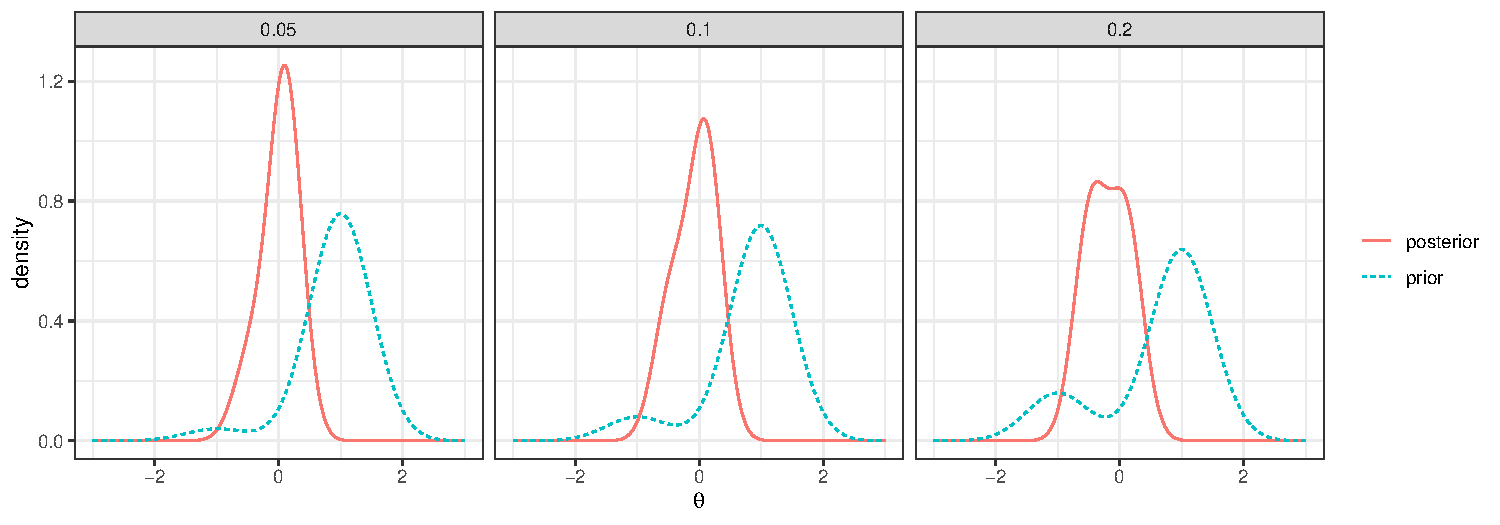
\includegraphics[width=1.15\linewidth]{figures/normal_mixture_prior_posterior.pdf}
\end{figure}

\scriptsize
\begin{minted}{R}

library(tidyverse)

y_bar = -0.25

post_mean_1 <- (0.25*y_bar + 0.1*1)/0.35
post_mean_2 <- (0.25*y_bar + 0.1*(-1))/0.35
post_std <- sqrt(1/14)

posterior_pi <-  function(pi) {
        pi*dnorm(y_bar,-1.0,sqrt(0.35))/((1-pi)*dnorm(y_bar,1.0,sqrt(0.35)) + pi*dnorm(y_bar,-1.0,sqrt(0.35))) }

plot_df_fun <- function(pi){
          data.frame(theta = seq(-3,3, length=1000)) %>%
           mutate(prior = (1-pi)*dnorm(theta, 1, 0.5) + pi*dnorm(theta, -1, 0.5),
                  posterior_pi = posterior_pi(pi),
                  posterior = (1-posterior_pi)*dnorm(theta, post_mean_1, post_std) +
                                  posterior_pi*dnorm(theta, post_mean_2, post_std),
                  pi=pi)}

plot_df <- bind_rows(lapply(c(0.2, 0.1, 0.05), plot_df_fun))

plot_df <- pivot_longer(plot_df, -c(theta,pi,posterior_pi), names_to="distribution", values_to="density")

ggplot(plot_df, aes(x=theta, y=density, col=distribution, linetype=distribution)) +
       geom_line() +
       xlab(expression(theta)) +
       theme_bw() +
       facet_grid(.~pi) +
       theme(legend.title=element_blank())
\end{minted}
\normalsize

\item This problem asks for an explicit expression of the mode of $\theta \mid \bar{y}$. It is just the $\argmax$ of the density in~\eqref{eq:bary_posterior}, which is easy to compute numerically. I do not think there is an analytic solution to the mode; indeed as per the figure above we see that the posterior could be bimodal as well. Here are a few things we can say (which we can verify e.g., by taking the derivative of the objective): the mode(s) must lie in $(\tilde{\mu}_2, \tilde{\mu}_1) = (-6.5/14, 1.5/14)$. Furthermore, as $\pi \to 0$, the mode converges to $1.5/14$ (I believe the answer the question writer was going for was $1.5/14$ and they meant to ask for an approximation of the posterior mode when $\pi$ is small). If you enjoy these kinds of calculations, also see~\citet{behboodian1970modes}.


\end{enumerate}

\subsection*{Problem 4: Assessing a clinical trial's conclusion}

Key ideas/tools:
\begin{itemize}
  \item Interaction effects in linear models.
  \item Intent-to-treat analyses.
  \item p-value interpretation.
\end{itemize}



\begin{enumerate}[label=(\alph*)]
\item Let us describe our main points of disagreement/agreement with the study:

\paragraph{Patients that dropped out:} A major issue with this study are the 51 patients that dropped out. If they had not dropped out, we would have a randomized experiment, and could even draw causal conclusions out of the two-sample comparison. Now, instead, we need to assume that the dropout of these patients was independent of their counterfactual (i.e., the response we would have observed, had they remained in their study). This may not be true, e.g., perhaps for some patients the drug has an adverse effect, and actually increases their blood glucose level. If these are these patients that dropped out, then the causal conclusions of the study will be flawed.

These situations arise all the time in medical studies, e.g., indeed, if a medication has side-effects on a patient, then it is not reasonable to expect them to keep taking that medication. However, there is a well-known remedy used: the investigators could have measured the glucose level at the end of the trial also for the patients that stopped taking the medication. Then we would use the measured response for these patients in an analysis, pooling them together with other treated patients. Such an analysis would produce an unbiased estimate of the treatment effect that however accounts for the (lack of) adherence of patients to the medication. This is called an \textbf{Intention-To-Treat  (ITT)} effect.

Unfortunately, here it seems the investigators did not/could not collect such intention-to-treat data. I would do a few sanity checks here (and perhaps report them as a sensitivity analysis in the manuscript's supplement): one check would be to conservatively ``impute'' a value for the patients that dropped out, say with $0$ (no change in glucose level), and rerun all analyses. If conclusions hold up even under a ``conservative'' , then we would be more confident in them. Another potential check would be to check if dropout is correlated with other patient-level variables (in case such data is available).

\paragraph{Reported effect and p-value:} The authors write that ``This study shows that the drug reduces glucose levels in subjects with moderately high glucose levels by more than placebo (t-test, $p < 0.0001$)'': It seems that this sentence refers to the two sample t-test that had a p-value of $0.0004$ which is not $< 0.0001$. Nevertheless, I mostly agree with this statement: modulo the patient drop-out considerations above, both the regression analysis and the two sample t-test support the conclusion that the drug reduced glucose level.

\paragraph{Interaction effects:} The authors further write that ``[the regression analysis] reveals that the drug is more effective in males than in females'': The coefficient for `sex` is not correctly interpreted here. The coefficient for `sex` hints that the decrease in glucose was stronger for males than females; across \emph{all} study subjects (i.e., whether treated or not). However it does not say anything about the relative effectiveness of the drug according to sex. The same erroneous interpretation is also applied to all other coefficients. Instead, one could try to answer the type of question asked here by including interaction effects in the regression, for example, \texttt{treatment * sex}. 

\paragraph{Study population:} The authors write ``we recommend that this drug be prescribed to every patient who wants to lower his/her glucose level." Critically, the study did not include diabetic patients who have high glucose levels and may be the most interested in taking the drug. Thus, recommending the drug to all potential patients seem premature without further study in this group. Even within the study population, the authors have not sufficiently backed up this claim. For example, they haven't shown evidence that the drug should be prescribed to both males and females, but they could easily add this evidence by conducting two t-tests, or fitting their regression model with an interaction term \texttt{treatment * sex}, and checking that the magnitude of the interaction term is smaller than the magnitude of the overall treatment effect.

\item Let us first outline concerns with the new study. In short, I do not believe the new study contradicts the first study.
\paragraph{p-values and power:} The major problem with this new study is that it misinterprets the p-value, i.e., it conflates the absence of evidence with the evidence of absence. While a small p-value provides evidence that we can reject the null hypothesis, a large p-value is uninformative: the p-value could be large either because the null is true or because the study is not powered sufficiently. Indeed; we only have a 12 vs. 12 comparison; a much smaller sample size than the first study. Furthermore, note that the p-value is still somewhat small and the authors of the new study commit the aforementioned fallacy and furthermore over-interpret the arbitrary cutoff of 0.05.
\paragraph{Generalizability:} The study recruitment criteria are slightly different than in the original study (e.g., start glucose levels 95-110 vs 100-120 in the original study, similarly for age) and so the populations of the two studies are also slightly different. However, I would not be worried too much about this here.

On the other hand, up to the small sample size, this appears like a nice randomized study that furthermore does not suffer from the dropout of the original study. I would thus start by looking at the 95\% confidence interval for $\mu_x - \mu_y$ in the new study. Even though we know that it will cross $0$, it would be promising to compare it to the confidence interval of the original study. Indeed, I think it is likely that the new confidence interval could provide further evidence for the effect found in the first study. One could also try to combine the two treatment effect estimates through a small meta-analysis (or if raw-data is available, use both studies in the same linear regression).	 

\end{enumerate}

\subsection*{Problem 5: Two ways of bootstrapping}
Key ideas/tools:
\begin{itemize}
  \item Time-series bootstrap.
  \item Bootstrapping individuals.
\end{itemize}

Statistician A's procedure does not make sense to me; there are some details missing from the description. Thus I think that this problem is quite open-ended and that the answer will depend on the interpretation of what Statistician A actually intends to do. Just make sure to describe in detail how you interpreted Statistician A, before providing an answer! In this solution we will assume that A's suggestion is to re-sample swimmer's with replacement.

One way to conceptualize what is going on, is as follows: there are two sources of variation in this dataset. First, swimmers are different from each other. Second, the time series measurements (i.e., the speed of the swimmers on 40 consecutive days) are also random; even when we only look at a single swimmer: each time they swim, there's a random source of variation determining how long it will take them to finish the 100 meters; and furthermore there is correlation across days: there could be hot-streaks, so that if a swimmer swims faster than expected on one day, they do so the next day too because of increased morale.

One way to formalize the two sources of randomness is through a hierachical model. First, for $i=1,\dotsc,100$ ( the 100 swimmers), we draw:
\begin{equation}
\label{eq:level1}
F_i \simiid \mathbb P,
\end{equation}
where $F_i$ is itself a probability measure on say $\RR^{41}$ and $\mathbb P$ is a probability measure on the space of probability measures. Here we assume that all the swimmers come from the same population that is described by $\mathbb P$.  At the second level of sampling, we draw for the $i$-th swimmer
\begin{equation}
\label{eq:level2}
(S_{it})_{1 \leq t \leq 41} \mid F_i\;\;  \sim \;\;F_i,
\end{equation}
and the statistician gets to observe $S_{it}, 1\leq t\leq 40$ and seeks to predict the $S_{i,41}$. 

Let us make this concrete by a simple random effects model. Say the only thing that differs across swimmers is the their mean speed $\mu_i$. Then the sampling could be described by the two-level model:
$$ \mu_i \sim \mathcal{N}(\nu, \tau^2),\;\;  S_{i\cdot} \mid \mu_i \sim \mathcal{N}(\mu_i, \Sigma),$$
for some $\nu, \tau^2, \Sigma$. This is not necessarily a good model, but it illustrates the more general two-level model described above; here the random distributions $F_i$ are equal to $F_i = \mathcal{N}(\mu_i, \Sigma)$. 


The difference between the two statisticians now can be described as follows: Statistician A  cares about the uncertainty induced from the sampling step in~\eqref{eq:level1}, while statistician B about the randomness in~\eqref{eq:level2}. 

Let us first discuss the two approaches assuming the model used to predict the 41st day is fixed and not trained based on the data at hand.

If we care about each swimmer individually, and want to assess uncertainty of the prediction individually for each swimmer, then we should follow the recommendation of Statistician B.\footnote{As an aside, it is perhaps worth noting a peculiarity in a time-series bootstrap when viewed in light of~\eqref{eq:level2}. We seek to represent uncertainty in $F_i$ based on a \emph{single} sample from $F_i$! This is only possible under strong assumptions, e.g., a parametric model assumption or the assumption that measurements taken multiple days apart are approximately independent.}

We would prefer an approach that samples swimmers (as suggested by Statistician A) if we care about the population of swimmers. For example, we could answer the following question: What is the average predicted speed across all possible swimmers in our population and what is our uncertainty? Then, we could resample swimmers with replacement (i.e., get $(S_{i_j\cdot})_{1\leq j \leq 100}$ with $i_j \in \cb{1,\dotsc,100}$), get the prediction for each, average these predictions to get an average prediction. We could repeat the sampling step multiple times and finally report a bootstrap percentile interval.

The suggestion of statistician A would also makes more sense if the model is trained on the swimmers themselves. For simplicity, let us consider a leave-one-out prediction scheme in which we are interested in predicting the speed of swimmer 1 on day 41 and train a model based on the other 99 swimmers. Then, keeping the time-series of swimmer 1 fixed, there is still randomness in the prediction because of the random selection of the other 99 swimmers. We could assess this uncertainty by resampling the 99 swimmers with replacement, building a new model each time and predicting the final speed of swimmer 1. An alternative here would be to combine the approaches of statisticians A and B: we could resample the other 99 swimmers with replacement to build a new predictive model, then use the time-series bootstrap to resample the data of swimmer 1, and finally predict the final speed of swimmer 1. Such a scheme would account for both sources of uncertainty. 








\subsection*{Problem 6: Population LASSO}

Key idea/tools:

\begin{itemize}
  \item Approximating the population objectives through empirical averages.
  \item The LASSO fit depends only on $\boldX^\top Y$ and $\boldX^\top \boldX$.
  \item Decomposing a covariance matrix through the Cholesky factorization or its eigenvalue decomposition. 
\end{itemize}


In this problem we are interested in solving the population LASSO problem,
\begin{equation}
\label{eq:population_lasso}
\argmin_{\beta} \frac{1}{2} \EE{\p{Y - X^\top \beta}^2} + \lambda \Norm{\beta}_1,
\end{equation}
where $(X,Y)$ are centered and have a known covariance matrix $\Sigma$. Instead, we have at our disposal a LASSO solver for the empirical objective:
\begin{equation}
\label{eq:empirical_lasso}
\argmin_{\beta} \frac{1}{2} \Norm{\boldY - \boldX^\top \beta}^2_2 + \lambda \Norm{\beta}_1,
\end{equation}
where $\boldX$ is a $N \times p$ design matrix with rows $x_i^\top$ and $\bold{Y}$ a $N\times 1$ response vector with entries $y_i$.

\begin{enumerate}[label=(\alph*)]

\item  Upon expanding the square of the population mean-squared error, we find that
\footnotesize
\begin{equation}
\label{eq:lasso_decomp}
\EE{\p{Y - X^\top \beta}^2} = \EE{Y^2 + \beta^\top  X X^\top  \beta -2 Y X^\top \beta} = \sigma_{YY} + \beta^\top \Sigma_{XX} \beta -2 \sigma_{XY}^\top \beta
\end{equation}
\normalsize
In particular, the solution of the optimization problem only depends on the covariance $\Sigma$ of $(X,Y)$. So for $i=1,\dotsc,N$ we could draw samples $(x_i, y_i)$ from a multivariate normal distribution with mean $0$ and the given covariance $\Sigma$. Then we could solve:

\begin{equation}
\label{eq:sample_lasso}
\min_{\beta} \frac{1}{2 N} \sum_{i=1}^N \p{y_i - x_i^\top \beta}^2 + \lambda  \Norm{\beta}_1
\end{equation}
For large enough $N$, by the law of large numbers, this would provide a good approximation to the population LASSO objective, since:
$$  \frac{1}{N} \sum_{i=1}^N \p{y_i - x_i^\top \beta}^2 \approx  \EE{y_i - x_i^\top \beta}^2, $$
where in light of~\eqref{eq:lasso_decomp} the approximation can be made uniform in $\beta$ (say for $\beta$ in a compact set; and we can check that for $\lambda > 0$ the optimal $\beta$ for the population problem indeed lies in a compact set). 

To use our friend's software we would use the pairs $(x_i, y_i)$ as input and set the penalty parameter to $N \cdot \lambda$. 

Let us provide a few more details on drawing samples from the specified multivariate normal distribution. Let $\Sigma = LL^\top$ be the Cholesky decomposition of $\Sigma$\footnote{Instead of the Cholesky decomposition, we could have have used the Eigendecomposition $\Sigma = VD^2V^\top$ and then proceeded as above with $L=VD$.} Then let $u_i^j \simiid \mathcal{N}(0, 1),\; j=1,\dotsc,p+1$, $u_i = (u_i^1, \dotsc, u_i^{p+1})$ and set:
$$ (x_i, y_i) = z_i = Lu_i$$
Then indeed $(x_i, y_i) \sim \mathcal{N}(0, \Sigma)$.
\item This question is phrased in a somewhat confusing way. My interpretation is as follows: let us assume we can solve~\eqref{eq:sample_lasso} exactly, i.e., let us ignore floating point arithmetic errors. Then, can we use~\eqref{eq:sample_lasso} to exactly solve~\eqref{eq:population_lasso}? It turns out that we can achieve this with what amounts to the computational shortcut for kernel learning~\citep{hastie2004efficient} when $p>n$.

Let $\Sigma = LL^\top$. This could be for example the Cholesky decomposition of $\Sigma$ (as explained for sampling in part a; also see footnote therein). Then let $\boldY$ be the last row of $L$ and $\boldX^\top$ the $p \times p+1$ matrix consisting of the first $p$ rows of $L$. We can think of this procedure as providing as with pseudoobservations $(x_i, y_i)$.

Note that by expanding as we did in~\eqref{eq:lasso_decomp} for the population objective, we get
\begin{equation}
\label{eq:sample_lasso_expanded}
 \Norm{\boldY - \boldX^\top \beta}^2_2  = \Norm{\boldY}_2^2 -2\boldY^\top \boldX\beta + \beta \boldX^\top \boldX\beta 
\end{equation}

However, by construction, we have that $\boldX^\top \boldX = \Sigma_{XX}$,  $\Norm{\boldY}_2^2 = \sigma_{Y}$ and $\boldX^\top \boldY = \sigma_{XY}$, so that these problems are the same.

\end{enumerate}
